\documentclass[a4paper]{article}

\usepackage{amsmath}
\usepackage{amsthm}
\usepackage{amsfonts}
\usepackage[utf8]{inputenc}
\usepackage{csquotes}
\usepackage{listings}
\usepackage{graphicx}
\usepackage{ifthen}
\usepackage{xspace}
\usepackage{hyperref}
\usepackage{mathtools}
\usepackage{tikz}
\usepackage{caption}
\usepackage{subcaption}

\DeclarePairedDelimiter\ceil{\lceil}{\rceil}
\DeclarePairedDelimiter\floor{\lfloor}{\rfloor}

\newcommand{\pgap}{~\\\noindent}

\newcommand{\Fsh}{{F$\sharp$}\xspace}

\newcommand{\col}[2]{{\begin{pmatrix} #1 \\ #2 \end{pmatrix}}}
\newcommand{\mmod}{\text{ mod }}

\newtheorem{theorem}{Theorem}
\newtheorem{lemma}{Lemma}
\newtheorem{definition}{Definition}

\lstset{basicstyle=\small\ttfamily,frame=leftline,numbers=left,xleftmargin=0.7cm,basewidth=0.14cm}
\lstset{rangeprefix=(*, rangesuffix=*),includerangemarker=false}

\lstnewenvironment{Code}{}{}
\newcommand{\codeInput}[2][]{\ifthenelse{\equal{#1}{}}{\lstinputlisting[title=#2]{#2}}{\lstinputlisting[linerange=#1-end,title=#2\ -\ #1]{#2}}}
\newcommand{\code}{\lstinline}


\title{POP 11g}
\author{Patrick Hartvigsen, Carl Dybdahl, Emil Søderblom}

\begin{document}

\maketitle

We have made an visual simulation of our solar system and compared the simulated data with the data from JPL Ephemeris.

\section{Design and Architecture}

\subsection{Architecture}

Figure \ref{uml} shows the UML diagram we made for this task. 

\begin{figure}[!ht]
\centering
%\includegraphics{uml.png}
\caption{The UML diagram for our architecture.}
\label{uml}
\end{figure}

\subsection{Algorithms}

For the task, we were only asked to do a first-order approximation of the movement of the planets, where we compute the acceleration and update the positions and velocities according to the following rules:

\begin{equation} \label{bad-p}
p(t_{n+1}) = p(t_n) + \Delta t \cdot v(t_n)
\end{equation}
\begin{equation} \label{bad-v}
v(t_{n+1}) = v(t_n) + \Delta t \cdot a(t_n)
\end{equation}

The precision of the simulation can, however, be significantly improved by using a second-order equation. For example, equation \ref{bad-p} can be improved with the following term:

\begin{equation} \label{good-p}
p(t_{n+1}) = p(t_n) + \Delta t \cdot v(t_n) + \frac{1}{2} \cdot \Delta t^2 \cdot a(t_n)
\end{equation}

The difference between equation \ref{bad-p} and \ref{good-p} is that \ref{bad-p} approximates the paths of the planets as locally linear, whereas \ref{good-p} approximates them as locally quadratic. Since the paths are curved, this approximation is much better in the long run.

In practice, however, the improvement does not make much of a difference, as equation \ref{bad-v} has the same imprecision as equation \ref{bad-p}. In order to get a true improvement, we compute the jerk, that is, the derivative of acceleration, so that we can also improve equation \ref{bad-v}. This gives us the following equation:

\begin{equation} \label{good-v}
v(t_{n+1}) = v(t_n) + \Delta t \cdot a(t_n) + \frac{1}{2} \cdot \Delta t^2 \cdot j(t_n)
\end{equation}

We wanted to compute the jerk using forward-mode automatic differentiation, but due to a limited type system in \Fsh this was not easily supported. Instead, we manually did the computations that an automatic differentiation algorithm would do.

In addition to this improvement in precision, we also allowed the sun to move and computed the effects of gravity from all bodies, not just the sun.

\section{Comparison with JPL Ephemeris}

We wrote a program, \code|JPLECompare|, which makes a table that compares our simulator to the JPL Ephemeris data. It outputs \code|csv|-formatted data to the standard output. We ran the program and produced the table \code|jplecompare.csv|.

While our results are not the exact same as JPL Ephemeris's data, only Mercury truly ends up out of sync with the rest of the solar system; some of the other planets end up in slightly different positions than they really should have, but rather than ending up with an entirely different orbit, they seem to merely be at a slightly different point in their orbit.

Figure \ref{comparison} contains a visual comparison showing that we don't lose much precision after 54 years of simulation.

\begin{figure}[!ht]
\centering

\begin{subfigure}{0.5\textwidth}
\centering
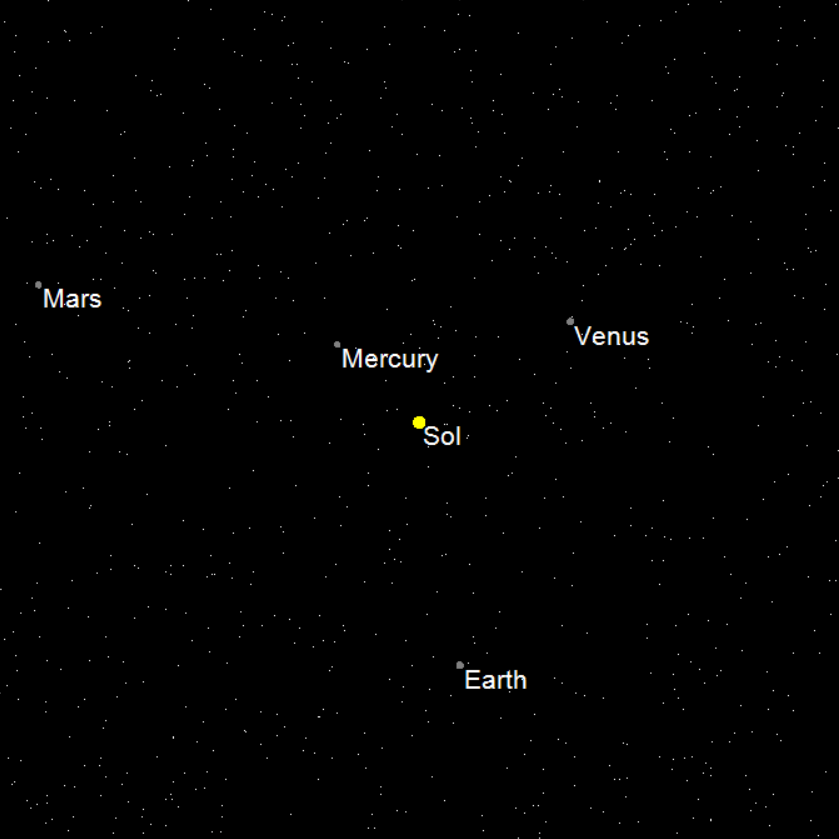
\includegraphics[width=0.8\linewidth]{comparison-our}
\caption{Our results after 54 years of simulation.}
\label{comparison:ours}
\end{subfigure}%
\begin{subfigure}{0.5\textwidth}
\centering
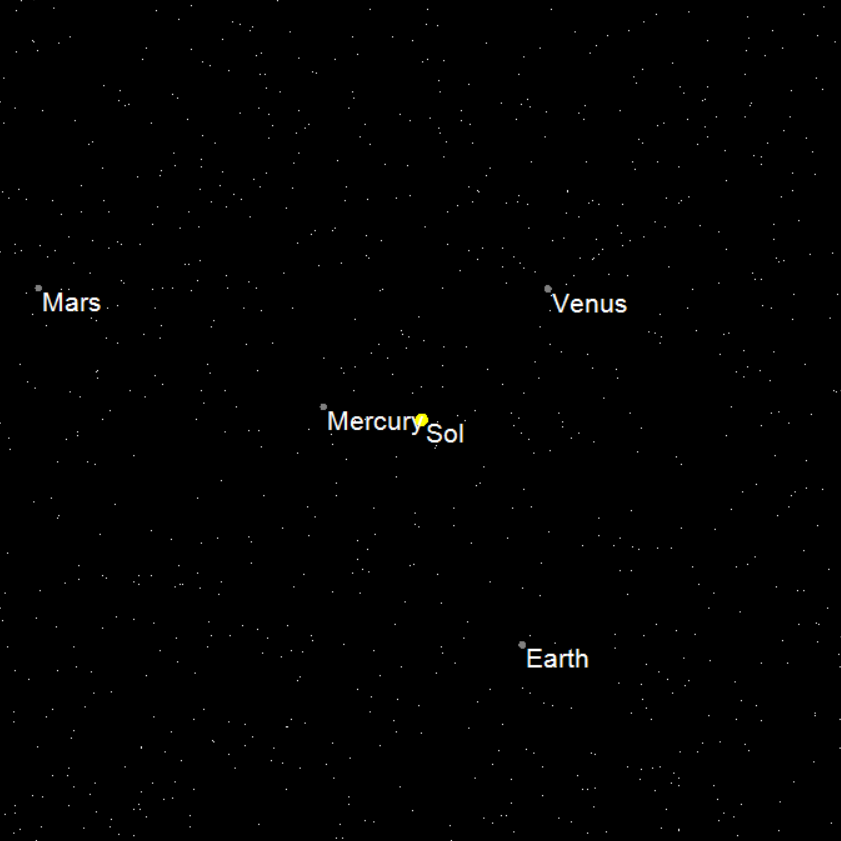
\includegraphics[width=0.8\linewidth]{comparison-jple}
\caption{JPL Ephemeris in 2016}
\label{comparison:jple}
\end{subfigure}

\caption{Comparison between our results, having simulated from 1962 to 2016, and JPL Ephemeris' results for the inner solar system. Sol is placed in the middle of each picture.}
\label{comparison}
\end{figure}

\section{Defects}

Because we compute the way each planet affects every other planet, our program is rather slow.

\end{document}	